\begin{exercice*}[Conditions nécessaires]
    Pour chaque figure ci-dessous, dire s'il est possible d'appliquer le théorème de Thalès.

    Justifier.
    \begin{multicols}4
        \begin{enumerate}
            \item \phantom{rrr}
            
            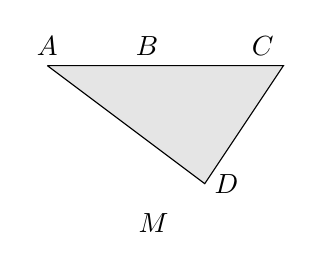
\begin{tikzpicture}[scale = 0.5]
                % \draw[help lines, color=black!30, dashed] (0,0) grid (7,6);        
                \coordinate[label=above:$A$] (A) at (1,5);
                \coordinate[label=above right:$B$] (B) at (3,5);
                \coordinate[label=above left:$C$] (C) at (7,5);
                \coordinate[label=right:$D$] (D) at (5,2);
                \coordinate[label=above right:$E$] (E) at (3.67,3);
                \coordinate[label=left:$M$] (M) at (4.33,1);
                \draw[fill=gray!20] (A)--(C)--(D)--(A);
                \tkzDrawLine[dashed, color=red, ultra thick](B,M);
                \tkzDrawLine[dashed, color=red, ultra thick](C,M);
            \end{tikzpicture}
            \columnbreak

            \item \phantom{rrr}
            
            \hspace*{-1cm}
            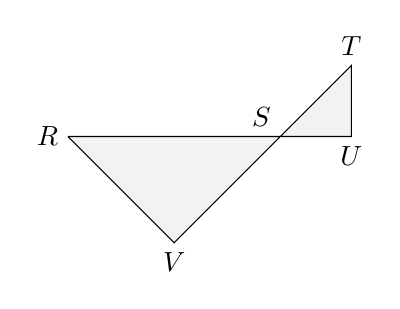
\begin{tikzpicture}[scale = 0.45]
                % \draw[help lines, color=black!30, dashed] (0,0) grid (10,7);        
                \coordinate[label=left:$R$] (R) at (1,4);
                \coordinate[label=above left:$S$] (S) at (7,4);
                \coordinate[label=above:$T$] (T) at (9,6);
                \coordinate[label=below:$U$] (U) at (9,4);
                \coordinate[label=below:$V$] (V) at (4,1);
                \draw[fill=gray!10] (R)--(S)--(V)--(R);
                \draw[fill=gray!10] (S)--(T)--(U)--(S);
                \tkzMarkRightAngle[fill=gray!60](S,V,R);
                \tkzMarkRightAngle[fill=gray!60](T,U,S);
            \end{tikzpicture}
            \columnbreak
            
            \item \phantom{rrr}
            
            \hspace*{-0.5cm}
            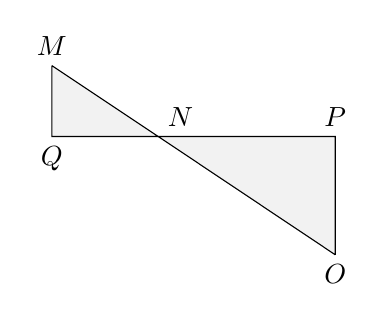
\begin{tikzpicture}[scale = 0.45]
                % \draw[help lines, color=black!30, dashed] (0,0) grid (10,7);        
                \coordinate[label=above:$M$] (M) at (1,6);
                \coordinate[label=below:$Q$] (Q) at (1,4);
                \coordinate[label=above right:$N$] (N) at (4,4);
                \coordinate[label=above:$P$] (P) at (9,4);
                \coordinate[label=below:$O$] (O) at (9,0.66);
                \draw[fill=gray!10] (M)--(N)--(Q)--(M);
                \draw[fill=gray!10] (O)--(N)--(P)--(O);
                \tkzMarkRightAngle[fill=gray!60](N,Q,M);
                \tkzMarkRightAngle[fill=gray!60](N,P,O);
            \end{tikzpicture}
            \columnbreak

            \item \phantom{rrr}
            
            \hspace*{-0.5cm}
            \begin{tikzpicture}[scale = 0.7]
                % \draw[help lines, color=black!30, dashed] (0,0) grid (6,5);        
                \coordinate[label=below right:$U$] (U) at (1,1);
                \coordinate[label=above left:$S$] (S) at (1.25,1.75);
                \coordinate[label=above right:$A$] (A) at (2,4);
                \coordinate[label=above:$F$] (F) at (2,1.43);
                \coordinate (F1) at (3,1);
                \coordinate[label=above:$G$] (G) at (5,2.72);
                \coordinate (G1) at (7.01,1.86);
                \coordinate (G2) at (8,4);
                \tkzDrawLine(U,A);
                \tkzDrawLine(U,G);
                \tkzDrawLine[dashed, color=red, ultra thick](S,F1);
                \tkzDrawLine[dashed, color=red, ultra thick](A,G1);                
                \pic[draw,angle radius=.5cm,angle eccentricity=1.5,"$\ang{30}$"] {angle=F1--F--G};
                \pic[draw,angle radius=.5cm,angle eccentricity=1.5,"$\ang{30}$"] {angle=G1--G--G2};
            \end{tikzpicture}

        \end{enumerate}
    \end{multicols}    
\end{exercice*}
\begin{corrige}
    %\setcounter{partie}{0} % Pour s'assurer que le compteur de \partie est à zéro dans les corrigés
    \phantom{rrr}    
    % \begin{multicols}2
        \begin{enumerate}
            \item Dans cette configuration, il n'y a pas de droites parallèles or c'est l'une
            des conditions nécessaires à l'application du théorème de Thalès.
            \item Dans cette configuration, il n'y a pas de droites parallèles or c'est l'une
            des conditions nécessaires à l'application du théorème de Thalès.
            \item Les droites $(MQ)$ et $(OP)$ sont toutes les deux perpendiculaires à la droite $(PQ)$, elles sont donc parallèles.
            
            Les droites $(MO)$ et $(PQ)$ sont sécantes en $N$.

            Donc toutes les conditions nécessaires à l'application du théorème de Thalès sont réunies.
            \item Les droites en pointillés rouges forment avec la sécantes $(UG)$ des angles
            correspondants égaux, elles sont donc parallèles.

            Les droites $(AS)$ et $(GF)$ sont sécantes en $U$.

            Donc toutes les conditions nécessaires à l'application du théorème de Thalès sont réunies.
        \end{enumerate}
    % \end{multicols}
\end{corrige}

